%  This LaTeX template is based on T.J. Hitchman's work which is itself based on Dana Ernst's template.  
% 
% --------------------------------------------------------------
% Skip this stuff, and head down to where it says "Start here"
% --------------------------------------------------------------
 
\documentclass[12pt]{article}
 
\usepackage[margin=1in]{geometry} 
\usepackage{amsmath,amsthm,amssymb}
\usepackage{graphicx}
\usepackage{tikz}
\usepackage{hyperref}
\usepackage[toc,page]{appendix}
\usepackage{gensymb}
\usepackage{tikz-3dplot}
\usetikzlibrary {3d} 

\newcommand{\iu}{{i\mkern1mu}}
\begin{document}
 
% --------------------------------------------------------------
%
%                         Start here
%
% --------------------------------------------------------------
 
\title{Quaternions: Revolve Around Something Luminous} % replace with the problem you are writing up
\author{Grant} % replace with your name
\maketitle

\subsection{Motivation}
Suppose you are making a game in 3D and you want to deal with 3D rotations. A natural way to do this would be to use \href{https://en.wikipedia.org/wiki/Euler_angles}{Euler angles}, with 3 angles telling us how to pitch, yaw, and roll. However, this representation of 3D orientation and rotation has problems: You can rotate yourself into a spot where you're stuck because of \href{https://en.wikipedia.org/wiki/Gimbal_lock}{Gimbal Lock}. If you try to rotate in a straight path between two orientations, say to make a character turn and look at something, interpolating Euler angles will produce strange paths. You will first rotate in random directions before going where you want to go. The solution is a 3D version of the complex numbers: quaternions. Understanding quaternions will convince you that rotations are actually very cursed, and you will even have a better understanding of imaginary numbers. There are so many interesting details to think about as you learn.

\subsection{2D: Complex Numbers}

First, let's consider how 2D rotations work using normal complex numbers. The square root of -1 may seem totally irrelevant to rotations, but if you think of complex numbers as vectors in a 2D plane, multiplying complex numbers corresponds to rotating the vectors. Consider what multiplying by $i$ does geometrically:

\begin{figure}[h]
    \centering
    \begin{tikzpicture}
        \draw[<->] (-1, 0) -- (1, 0);
        \draw[<->] (0, -1) -- (0, 1);
        \draw (1,0) node[anchor=west] {$1$} (0,1) node[anchor=south] {$i$} (-1,0) node[anchor=east] {$-1$} (0,-1) node[anchor=north] {$-i$};
        \draw[->] (0.5,0) arc (0:85:0.5);
        \draw[->] (0,0.5) arc (90:175:0.5);
        \draw[->] (-0.5,0) arc (180:265:0.5);
        \draw[->] (0,-0.5) arc (270:355:0.5);
    \end{tikzpicture}
    \caption{Multiplying by $i$ is a $90\degree$ counterclockwise rotation: $1 \times i = i\,(90\degree), i \times i = -1 \,(180\degree),-1\times i = -i\, (270\degree),-i \times i = 1 \,(360\degree)$}
    \label{complexplane}
\end{figure}


This also works for any arbitrary complex number $a + b \iu$, as $b - a \iu$ is precisely that vector rotated $90\degree$ counterclockwise. Check to see if you can verify this by drawing the vectors yourself. This fact, along with the fact that $e^x$ is its own derivative, actually gives us a way to derive Euler's formula:
\[
e^{i\theta} = \cos(\theta) + \iu \sin(\theta)
\]

The function $e^{i\theta}$ traces out a unit circle in the complex plane at a constant velocity! Here, you should not think of $e^x$ as exponentiation in the repeated multiplication sense at all, but in the "function that is its own derivative" way only. You should remind yourself how you derived this from the Taylor series in calculus (\ref{appendix:eixtaylor}), but freshman physics also gave you another way to think about it: uniform circular motion. 

Recall that in uniform circular motion, the acceleration was always perpendicular to velocity, and velocity was perpendicular to the displacement from the center of the circle. Thus, all 3 of those vectors changed direction, but not magnitude. The same thing is happening with $e^{i\theta}$:
\[
f(\theta) = e^{i\theta}
\]
\[
f'(\theta) = i f(\theta)
\]

Because multiplying by $i$ is a $90\degree$ rotation, $f'(\theta)$ will always be "perpendicular" to $f(\theta)$. If we think of $f(\theta)$ as displacement from center and $f'(\theta)$ as velocity, we can see why $f(\theta)$ traces out a unit circle starting from $f(0) = e^0 = 1$:

\begin{figure}[h]
    \centering
    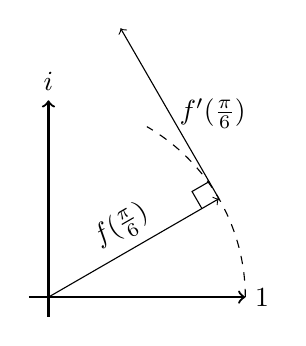
\begin{tikzpicture}[scale=2.5]
        \draw[thick,->] (-0.1, 0) -- (1, 0);
        \draw[thick,->] (0, -0.1) -- (0, 1);
        \draw (1,0) node[anchor=west] {$1$} (0,1) node[anchor=south] {$i$};
        \draw[->] (0, 0) -- (0.866025, 0.5) node[midway,sloped,above] {$f(\frac{\pi}{6})$};
        \draw[->] (0.866025, 0.5) -- (0.366025, 1.36603) node[midway,right] {$f'(\frac{\pi}{6})$};
        \draw (0.779423, 0.45)-- (0.729423, 0.536603) --(0.816025, 0.586603);
        \draw[dashed] (1,0) arc (0:60:1);
    \end{tikzpicture}
    \caption{$f(\theta)=e^{i\theta}$ is undergoing uniform circular motion.}
    \label{uniformcircular}
\end{figure}

How does this help with our goal of showing how multiplication corresponds to rotation? With Euler's formula, we can now say that we have access to all the properties of exponents! Instead of writing a complex number $z = x + y\iu$ using the $x$ and $y$ coordinates in the Cartesian plane, we can instead use the magnitude $a$ and the angle $\alpha$ to write $z = a e^{\iu \alpha}$. Thus, $e^{i \theta} z = a e^{\iu (\alpha + \theta)}$, which corresponds to $z$ being rotated by $\theta$ radians counterclockwise!

Armed with all this, we have these deeper/more useful/more concrete ways for thinking about $i$ than simply $i = \sqrt{-1}$. Now, to take it another step further and explain how $i$, or a $90\degree$ rotation, is actually a bivector, let's step up to 3D quaternions! 

\section{3D: Quaternions}
In 3D, there are three planes that you can rotate in (or, equivalently, three axes you can rotate around, if you want to think about the normal vectors of those planes). Thus, we now need three imaginary units: $i$, $j$, and $k$. $i$ could be rotation in the yz plane, $j$ could be rotation in the -xz plane, and $k$ could be rotation in the xy plane. In 2D, $i$ represented the only "axis" that we could rotate around, but now it is just one of three. 

Additionally, rotating in 3D is not commutative, unlike in 2D. In 2D, rotating by $\theta$ and then by $\phi$ is the same as rotating by $\phi$ then $\theta$. You can reverse the order in which you apply rotation. However, you cannot do that in 3D: try rotating $90\degree$ in the xy plane and then rotating $90\degree$ in the yz plane. This rotation takes $\hat{x}$ to where $\hat{z}$ used to be, $\hat{z}$ to $-\hat{x}$, and $\hat{y}$ to $-\hat{x}$, but the reverse order takes $\hat{z}$ to $\hat{x}$, $\hat{x}$ to $\hat{y}$, and $\hat{y}$ to $\hat{z}$ (see if you can sketch or think this through with right-hand rule and hand contortions). This means that quaternion multiplication is \textbf{not} commutative anymore! That is, $ab \ne ba$ when $a$ and $b$ are general quaternions. 

Another property that the quaternion units should have is that they should square to $-1$ exactly like the original imaginary $i$. We want them to behave exactly like $i$ in the 2D planes that they are in charge of (their subspaces of the 3D space). This is a very hand-wavey justification, but please bear with me for the geometric algebra way of doing it.

\[i^2=j^2=k^2=-1\]

To upgrade Euler's formula to 3D, we can use $i$, $j$, and $k$ to specify an axis of rotation using a unit vector and replace the original $i$:

\begin{align*}
e^{i\theta} &= \cos(\theta) + i \sin(\theta) \\
e^{\theta (a i + b j + c k)} &= \cos(\theta) + \sin(\theta) (a i + b j + c k) \qquad (a^2 + b^2 + c^2 = 1)
\end{align*}\footnote{These formulae are actually very closely related to Lie algebras and Lie groups. The right hand side can be thought of as a point on a 2D sphere (aka circle) or a 4D sphere, and the thing in the exponential is an element of the space tangent to the sphere at the identity element. The tangent space (Lie algebra, imaginary line $\rm{Re}[z]=1$) is 1 dimension lower than the sphere (Lie group, unit circle).}

In order for this to work, notice that the value $ai + bj + ck$ must also square to $-1$ so that it can be treated like $i$. So far, we have not defined how to multiply $i$, $j$, and $k$ with each other, only themselves. It turns out that if the three units \emph{anti-commute} ($ij = -ji$ for any 2 of the 3 units), it will work out. Fun exercise for the reader! This anti-commutative property can be better explained using the geometric algebra approach, so for now just treat it as a fact handed down from up high. In the end, this quaternion multiplication table turns out to work. Note that the specific placement of the negative signs is just one convention (one that agrees with right-hand rule).

\begin{figure}[h]
    \centering
    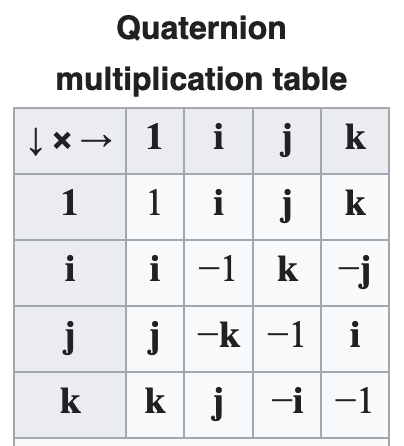
\includegraphics[width=0.25\linewidth]{multtable.png}
    \caption{$i^2 = j^2 = k^2 = ijk = -1$}
    \label{multtable}
\end{figure}

\newpage

To this point, I still have not explained how to rotate vectors using quaternion multiplication. 


\section{Appendix}
\begin{appendices}

\subsection{$e^{ix}$ with Taylor Series}
\label{appendix:eixtaylor}
This is the graph appendix...

\subsection{Another Appendix}

\end{appendices}



% --------------------------------------------------------------
%     You don't have to mess with anything below this line.
% --------------------------------------------------------------
 
\end{document}